\usetikzlibrary{arrows.meta}
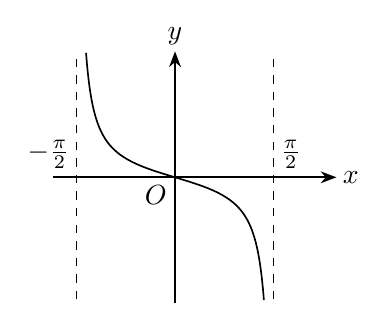
\begin{tikzpicture}[x=1cm,y=1cm,line width=.6pt,font=\normalsize,>=Stealth]
\draw[dashed] (-1.25,-1.55)--(-1.25,1.55);
\draw[dashed] (1.25,-1.55)--(1.25,1.55);
\draw[domain=-1.42:1.42,samples=201] plot ({0.7958*\x},{-0.24*tan(\x r)});
\draw[->] (-1.55,0)--(2.05,0) node[right,inner sep=0pt,xshift=2pt] {$x$};
\draw[->] (0,-1.60)--(0,1.60) node[above,inner sep=0pt,yshift=2pt] {$y$};
\node[anchor=north east,inner sep=1pt] at (-0.06,-0.06) {$O$};
\node[anchor=south east,inner sep=0pt] at (-1.33,0.10) {$-\frac{\pi}{2}$};
\node[anchor=south west,inner sep=0pt] at (1.33,0.10) {$\frac{\pi}{2}$};
\end{tikzpicture}
